\documentclass[a4paper]{article}		%Basic Document class: article
\usepackage[english]{babel}			%Babel
\usepackage{url}				%
\usepackage{hyperref}				%Make Links clickable
\usepackage{graphicx}				%For Pictures, includegraphics[options]{name}
\usepackage{fancyhdr}				%For better headers

%%%%%%Setting up the header
\fancyhead{}						% clear all header fields
\chead{\bfseries Medical technology in smart cars}	%Print the ditle of the paper in every header, in the center
\renewcommand{\headrulewidth}{0.4pt}			%Make a line between the header and the content
\pagestyle{fancy}					%Use the fancy style from the package for the headers and footers

%%%%%Edit style of the document

%%%%%Set Title values
\title{									%Set all the data for the title page, which is created later in the document
	
\includegraphics[height=2cm]{images/higlogo}\\\vspace{1cm}	%vspace, vertical space of x cm to the next line
	Medical technology in smart cars\\\vspace{7mm}
	\Large{Project work of group 5}\\\vspace{5mm}			%Large, for a bigger font.
	\normalsize{Spring Semester 2015}\\\vspace{1cm}			
	\large{IMT 3591 Artificial Intelligence\\
		Gj\o{}vik University College
		\\\vspace{1cm}}}

%%%%%%Set author values
\author{			%Set the author, als included on the title page
Laodice Melliti\\
Matr.-Nr: 140159\\
{\tt laodice.melliti@hig.no}
\and 
Jonas Helbig\\
Matr.-Nr: 140165\\
{\tt jonas.helbig@hig.no}
\vspace{1cm}}

%%%%%%%%%%%%%%%%%%%%%%%%%%%%%%%%%%%%%%%%%%%%%%%%%%%%%%%%%%%%%%%%%%%%%%%%%%%%%%%%
%
%Acctual begin of the document
%
%%%%%%%%%%%%%%%%%%%%%%%%%%%%%%%%%%%%%%%%%%%%%%%%%%%%%%%%%%%%%%%%%%%%%%%%%%%%%%%%

\begin{document}	
\maketitle				%Make title page
\thispagestyle{empty} 	%remove the page number
\begin{abstract}		%Short abstract on the title page
	This document is part of our project for the course Artificial Intelligence at Gj\o{}vik University College. This paper describes the architecture and framework of a system which helps elderly and/or people with chronic illnesses, with detection and prevention of potential harmful incidents while driving a car. 
\end{abstract}

\newpage				%Continue on a new page
\tableofcontents		%Generate table of contents
\newpage
%%%%%%%%%%%%%%%%%%%%%%%%%%%%%%%%%%%%%%%%%%%%%%%%%%%%%%%%%%%%%%%%%%%%%%%%%%%%%%%%
%End of title page and Table of contents, the actual content comes
%%%%%%%%%%%%%%%%%%%%%%%%%%%%%%%%%%%%%%%%%%%%%%%%%%%%%%%%%%%%%%%%%%%%%%%%%%%%%%%%
\section{Formal}
Group number: 5\\
Names of the group members: Laodice Melliti, Jonas Helbig\\
Contribution of Laodice Melliti: System 3, Our system, system architecture - graphic\\
Contribution of Jonas Helbig: System 1, system 2, Our system \\
\section{Introduction}
\indent					%Dirty fix, to indent the first line in each section. 
\indent Throughout this paper, we will design an AI system, which could later be implemented in a smart car application. The primary goal of the system is to assist elderly or sick people during everyday driving situations.

We begin this paper with a look at  the state of art in the area of in-car vital parameter monitoring. We give a short overview and look at three systems in more detail. Afterwards, we introduce and describe our proposed system.
\section{State of the art}
\indent
\indent Apart from systems designed to prevent drunk driving or systems with eye recognition that detect if the driver falls asleep, there are surprisingly few public used or commercially available systems in the area of in-car vital parameter monitoring. Therefore, we focus here on research done in this area. In \cite{schneider:12}, the authors research on the validation of electrocardiography (ECG) measurement in a car-integrated test framework.

In \cite{eilebrecht:12} the authors describe the relevance of the heart rate variability (HRV), extracted from the ECG, for driver workload detection in real world driving.

In \cite{walter:11} the authors describe the development and testing of a smart cart seat to measure vital signs with non-contact methods.

In the next three sub sections we describe the work in \cite{yamakoshi:07}, \cite{Zocchi:07} and \cite{angelo:10} in more detail.
\subsection{System 1}
\indent
\indent In the paper \cite{yamakoshi:07} the authors describe the effects of long monotonous driving in a simulated session. Their architecture consists of several sensors that measure different vital parameters like skin temperature, peripheral resistance and normalized pulse volume. As actuators, they use a display for real-time monitoring and they save the data for offline-analysis.
The system itself only measures and presents the data, without taking further actions based on it.
\subsection{System 2}
\indent
\indent In the paper \cite{Zocchi:07}, the authors use a system of sensors to find correlations between vital parameters like galvanic skin resistance, peripheral temperature and heart rate variability to determine the psychophysical state of the driver. This is especially for sleep attacks and micro-sleeps detections. The architecture consists of several sensors for vital parameter measurement. The actuators consist of a display and several computers to see the data in real-time and to save the data for later analysis. Their long-term goal is to develop a learning agent system which adjusts itself over time to the person usually monitored.
\subsection{System 3}
\indent
\indent In the paper  \cite{angelo:10}, the system calculates the driver`s stress level by measuring his vital signs. The sensors are integrated in the car, mainly in the steering wheel. The car displays the results at the driver`s demand and, depending on the results, can adjust the music`s volume and/or block incoming phone call.

\section{Our proposed System}
\indent
\indent Our system, the smart car, is to assist sick and/or elderly people when they need to drive by regularly checking their health.
To do so, we will implement sensors in the car to measure heart rate, blood pressure and skin resistance. By using the gathered data, the car calculates the stress level, the state of consciousness and the general health of the driver. With that, it can warn the driver to, depending on the situation, consider an appointment with a doctor or to call an ambulance. If the driver has too poor health, the car will first ask whether to call for an ambulance or not. If no answer is given, then it will call the ambulance anyway. If, once the call is made, the driver does not talk, the car will send the coordinate using the data from the GPS.
\subsection{PEAS Description}
\paragraph{Performance} The car needs to be able to detect when the driver`s state is harmful for himself and/or other (for example, if the blood pressure is too low there is a risk of losing consciousness) and to warn the driver of his condition.

\paragraph{Environment} For this project, we only consider the driver, the car (which includes all the built in material) and two external devices (heart belt and pressure sensor) which will be further explained in the next paragraph. The environment outside of the car does not influence this system and we assume that the data is not invalidated by the driver`s clothes.

\paragraph{Actuators} We have three actuators. First, a mobile phone which is built in the system. It will call the ambulance if needed. Secondly, speakers that are built in too. We are using the radio speakers. If the driver is listening to it, then the car will overwrite it in case of an emergency. Thirdly, an interface (touch screen) placed next to the radio that can display what the car say.

\paragraph{Sensors} We have three sensors for medical data and two other kinds of sensors. For the medical data, both the blood pressure and the heart beats will be sensed using an external device. We will use a blood pressure meter and a “heart belt” for the heart pressure. Those devices will be put directly against the driver`s skin. As for the skin resistance, we will put the sensors on the stirring wheel. Supposing that the driver drives normally and without gloves, then we can read the data from the tip of the finger (which is the best). The last two sensors are a GPS, either built in the car or from a mobile phone, and the touch screen. The last one is used by the driver to interact with the car (for example when it asks to call for an ambulance).

\subsection{System architecture}
\begin{figure}[h!]
	\centering
	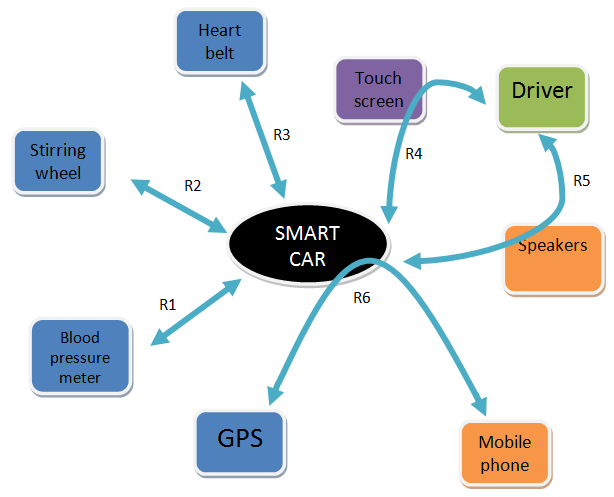
\includegraphics[scale=0.5]{./images/architecture}		%Include picture
	\caption{System Architecture}					%Picture caption
	\label{fig:sys}									%Label of the picture, can be referenced with \ref{fig:sys}
\end{figure}
Our system architecture is presented in Figure \ref{fig:sys}.
\begin{description}\addtolength{\itemsep}{-0.5\baselineskip}
	\item{R1:} The blood pressure meter gets the blood pressure’s data (sensor).
	\item{R2:} The stirring wheel gets the data about the skin resistance (sensor).
	\item{R3:} The heart belt gets the data about the heart rate (sensor).
	\item{R4:} The driver gives his answer using the touch screen (sensor \& actuator).
	\item{R5:} The smart car informs the driver of his state using the speakers (actuator).
	\item{R6:} The smart car calls an ambulance using a mobile phone (actuator).
	
	If needed, it uses the GPS coordinates (sensor).
\end{description}
\bigskip
\indent
\indent Our system`s main difference with the other existing project is that we reunite both the capacity to check the driver`s health and the capacity to call someone (here, the ambulance). The combination of this two functionalities has yet to be reunited in the same smart car.


\section{Formal: Assignment 2}
\textbf{Contribution of Laodice Melliti:} Implementation scope, algorithmic design and description, implemented system architecture graphic\\
\textbf{Contribution of Jonas Helbig:}  Implementation scope, algorithmic design and description\\
\section{Implementation scope}
\indent					%Dirty fix, to indent the first line in each section. 
\indent
The system as presented by us so far is too comprehensive to be fully implemented during this project. This section will give an estimation about which parts of the system can actually be implemented by us in the scope of this project.

Instead of focusing on emergency response systems with functions like detecting heart attacks, sleep attacks or even death during driving, we implement a system for long term measurement and monitoring of the user's health.
We focus on three different health values, namely the heart beat, the breathing rate and the blood pressure. Our system is intended to be used by elderly people or people with illnesses affecting one of those parameters. 
We create a system capable of detecting unusual or undesirable development of a persons health over a longer period of 30-100 days.

In short, our system will create long term trends on the development of the user's health status. While doing that it is smart enough to detect unusal values and assess them in cooperation with the user to reduce or increase their influence on the trend.
The process is further described below.
\begin{enumerate}
	\item For the initial setup of the training, we recommend the visit of a doctor. Since every patient has a different medical history, a doctor has to determine through several appropriate test the ``normal'' condition of the patient in reference to our desired parameters. Those are the boundaries used by our functions defined later. After the initial setup, the system will be activated every time the users uses his car.
	\item During each session the system will capture the parameters from the user, prepare and normalize the data and extract our desired features.
	\item The extracted features (as described later) will be processes by our system with the algorithms described in the next section.
	\item The system will react to unusual values, outside of the boundaries predetermined by a doctor in the first step and it will try to find reasonable explanations in cooperation with the user, with a predefined question catalog. The questions can be answered binary, so that the user could easily give feedback without being distracted while driving. 
	\item Depending on the responds of the user, the system will adjust its validation and weighting system for the calculation of the long term rating.
	\item Those ratings determined over a longer time will be repeatedly presented to the user, together with recommendations on how to react.
\end{enumerate}

To reduce the complexity and avoid handling raw medical data, we are only implementing the steps three to six. The other steps would be scope of further research and could for example focus on the practicality of this preparation and extraction.
From the different sensors and actuators described in the last section we are going to use the following ones:
\begin{itemize}
	\item Hear belt: From this sensor we use the heart beat rate and the breathing rate which is continuously measured. For our purpose, we assume that we get the values as heart beat per second and breaths per second.
	\item Blood pressure meter: From this sensor we use both the systolic and the diastolic blood pressure values. For our purpose, we assume that we get the values as millimeters of mercury. Since acquiring the blood pressure data can be distracting for the driver, we only measure them once every 30 minutes.
	\item GPS: For each dataset we save in the database we save the approximate GPS location. This could later be used to determine eventual correlations between the health status and the physical position of the user (for example often stress during driving on a highway).
\end{itemize}
Our implementation is summarized in figure \ref{fig:flow}.
\begin{figure}
	\centering
	\graphitemize{Get features,  Create long\\term trend, Modify weights, Ask user, Detect unusual\\ values}
	\caption{Process flow of our implementation}
	\label{fig:flow}
\end{figure}

\section{Algorithmic approach}
\indent					%Dirty fix, to indent the first line in each section. 
\indent
The pseudo code for our approach is specified through the algorithms \ref{alg:capture} and \ref{alg:longterm}.
We focus on the important functions and aspects, without going into details about the capturing and preparation of the data.
All the important functions and variables used are described below.
\begin{algorithm}[htbp]
	\begin{algorithmic}[1]
		\Require{None}
		\Ensure{Database, Session trend}
		\Repeat
		\For {five minutes}
		\State $capturedData \gets$ \Call{CaptureData()}{}
		\State $preparedData \gets$ \Call{PrepareData}{$capturedData$}
		\State $data \gets$ \Call{ExtractFeatures}{$preparedData$} \Comment{data: concrete numbers of BP/ BR and HB}
		\EndFor
		\State $median \gets$ \Call{Average}{$data$} \Comment{Average of the last 5 minutes}
		\State $GPScoordinates \gets$ \Call{GetGPS()}{}
		\State $weight \gets 1$  \Comment{Default value for the weighting function}
		\If {\Call{OutsideBoundaries}{$median$}}
			\State $response \gets$ \Call{AskUserQuestions()}{}
			\If {$response == yes$} \Comment{yes: valid reason for data out of boundaries}
				\State \Call{ReduceWeight()}{}
			\Else
				\State \Call{IncreaseWeight()}{}			\EndIf
		\EndIf
				
		\State \Call{Store}{$median$, $weight$, $GPScooridinates$} \Comment{Save values in Database}
		\Until{Driving session is over}
		\State \Call{SessionEvaluation()}{}	\Comment{Presented at the end of each driving session}
	\end{algorithmic}
	\caption{Capturing, processing and storing the data}
	\label{alg:capture}
\end{algorithm}
		%%%%%%%%
\begin{algorithm}[htbp]
	\begin{algorithmic}[1]	
		\Require Database
		\Ensure Recommendation for the user
		\Repeat
		\State $data \gets$ \Call{ReadDatabase()}{}
		\State $rating \gets 0$	
		\ForAll {$dataset$ in $data$} \Comment{every dataset consists of median, weight and gps}
		\State $rating \gets rating + dataset.weight * dataset.median$
		\EndFor
		\State $rating \gets rating / data.length$ \Comment{Average with weight}
		\If {\Call{OutsideBoundaries}{$rating$}}
			\State \Call{makeRecommendation()}{}
		\EndIf
		\Until{}
	\end{algorithmic}
	\caption{Long term monitoring}
	\label{alg:longterm}
\end{algorithm}

\paragraph{Detailed explanation for Algorithm \ref{alg:capture}}
\subparagraph{Functions:}
\begin{description}
	\item [CaptureData()] For the heart beat and breath rate : capture the data every second. For the blood pressure, capture the data every 30 minutes.
	\item [PrepareData(capturedData)] Normalization of the data received, reduction of the noise as much as possible and conversion from analog data into digital data.
	\item [ExtractFeatures(preparedData)] Extraction of the concrete values we use in the later steps of the algorithm.
	\item [Average()] Every 5 minutes, we make an average of all the data received.
	\item [GetGPS()] Get the current GPS position
	\item [OutsideBoundaries(median)] We check if the data is outside the boundaries (too high or too low in comparison to the patients optimal health state). Those boundaries are set up by a doctor when the system is implemented in the car. This function returns a boolean variable\\
	\underline{True} : The data is outside the boundaries\\
	\underline{False} : The data is inside the boundaries. In this case we assume everything is fine
	\item [AskUserQuestion()] We ask the driver if he had exerciced recently and if he is feeling unwell or stressed. If the answer to any of this questions is yes, then the function return a boolean variable set to true. Otherwise, it returns false.
	\item [ReduceWeight()] Set the weight to a number between zero and one. This later reduces the impact of the data to the long term trend. It is necessary to reduce the influence of abnormal data which has a valid reason.
	\item [IncreaseWeight()] Set the weight to a number above one. This later increases the impact of the data to the long term trend. It is necessary to increase the influence of abnormal data which does not have a valid reason.
\item [Store(median, weight, GPScooordinates)] We store the median, the weight and the GPS coordinates associated together into the database.
\item [SessionEvaluation()] We make an average of all the data received during the driving session so that we can compare two driving sessions with each other.
\end{description}

\subparagraph{Variables:}
\begin{description}
	\item [capturedData] The data captured by the sensors without any processing.
	\item [preparedData] The captured data is normalized, noise-reduced and converted to digital.
	\item [data] The concrete values used by our system during the later steps of the algorithms.
	\item [median] The average of 5 minutes of data.
	\item [GPScoordinates] Everytime we calculate the median, we acquire the GPS coordinates of the car. That way, it can be possible to make a correlation between the place and the driver's status.
	\item [weight] Importance given to a median. The default is one (neutral). If the median is out of boundaries and the driver says there is a reason for it (eg. : tiredness, stress, exercises,\dots ) then we reduce the weight. If there is no explanations for the median to be out of boundaries, then we increase the weight.
	
	
\end{description}
\paragraph{Detailed explanation for Algorithm \ref{alg:longterm}}
\subparagraph{Functions:}
\begin{description}
	\item [ReadDatabase()] We put a specific amount of data into a new variable to analyze them without accidentally changing our saved data.
	\item [OutsideBoundaries()] See functions of algorithm \ref{alg:capture}.
	\item [MakeRecommendation()] Depending of the result, we either make recommendation to see a Doctor (via speakers), we give the driver advices or we inform them that everything is fine.
\end{description}
\subparagraph{Variables:}
\begin{description}
	\item [data] Contain a certain amount of the database information.
	\item [rating] Used to calculate the average with weight of the data.
	\item [data.length] Length of the variable data which is an array.
	\item [dataset.weight] Value defined in algorithm \ref{alg:capture}.
	\item [dataset.median] Value defined in algorithm \ref{alg:capture}.
\end{description}
\newpage
\section{Updated system architecture}
\indent					%Dirty fix, to indent the first line in each section. 
\indent
\begin{figure}[h]
	\centering
	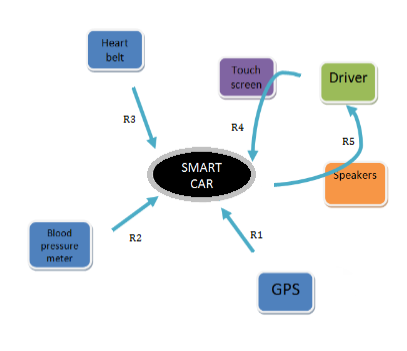
\includegraphics[scale=0.8]{./images/implementationArchitecture}		%Include picture
	\caption{System architecture redefined for the scope of our project}					%Picture caption
	\label{fig:impsys}									%Label of the picture, can be referenced with \ref{fig:impsys}
\end{figure}

\begin{description}\addtolength{\itemsep}{-0.5\baselineskip}
	\item{R1:} Get the GPS position
	\item{R2:} Get the extracted features for the blood pressure
	\item{R3:} Get the extracted features for the breathing rate and the heart beat
	\item{R4:} Receive responses from user
	\item{R5:} Ask user questions
\end{description}
\newpage	%Newpage for the references
%%%%%%%%%%%%%%%%%%%%%%%%%%%%%%%%%%%%%%%%%%%%%%%%%%%%%%%%%%%%%%%%%%%%%%%%%%%%%%%%
%End of the normal document, the Bibliography follows
%The Bibliography is generated from the example.bib file
% ---- Bibliography ----
%%%%%%%%%%%%%%%%%%%%%%%%%%%%%%%%%%%%%%%%%%%%%%%%%%%%%%%%%%%%%%%%%%%%%%%%%%%%%%%%
\bibliographystyle{ieeetr}  	%Set the style for the bibliography, after certain standards
\bibliography{bibliography}			%Automaticly create a bibliography

\end{document}
%End of the whole document, everything from here will be ignored
